\documentclass[12pt, aspectratio = 169]{beamer} % handout

\usepackage{amsmath} % Mathematics related packages
\usepackage{fontawesome} % 'fontawesome' font
\usepackage{ragged2e}
\usepackage{color}
\usepackage[round]{natbib}
\usepackage{tikz}

% For 'InkScape' integration
\usepackage{import}
\usepackage{xifthen}
\usepackage{pdfpages}
\usepackage{transparent}

\usetheme[]{metropolis}
\usecolortheme[]{wolverine}

\usefonttheme{serif}
\setbeamercovered{transparent = 0.5}

\setbeamertemplate{theorems}[numbered] 

\definecolor{title-bg}{RGB}{240, 240, 240} 
\definecolor{title-fg}{RGB}{128, 113, 93}
\definecolor{my-red}{RGB}{254, 132, 135}
\definecolor{my-blue}{RGB}{59, 180, 252}
\definecolor{my-green}{RGB}{125, 221, 149}
\definecolor{titles}{RGB}{0, 0, 112}

\setbeamertemplate{footline}{%
	\leavevmode%
	\hbox{%
		\begin{beamercolorbox}[wd = 0.800\textwidth, ht = 4ex, dp = 2ex, left]{}%
			\hspace{6pt} \texttt{Joint Statistical Meetings 2022.\phantom{|}August 10, 2022.}
		\end{beamercolorbox}%
		\begin{beamercolorbox}[wd = 0.120\textwidth, ht = 4ex, dp = 2ex, center]{}%
			\raisebox{-1pt}{\insertslidenavigationsymbol~\insertsectionnavigationsymbol}
		\end{beamercolorbox}%
		\begin{beamercolorbox}[wd = 0.080\textwidth, ht = 4ex, dp = 2ex, center]{}%
			\texttt{\insertframenumber~/~\inserttotalframenumber}
		\end{beamercolorbox}%
	}%
}%

% Personal Information
\author{André Victor Ribeiro Amaral \\ \href{mailto:andre.ribeiroamaral@kaust.edu.sa}{andre.ribeiroamaral@kaust.edu.sa}}

\begin{document}
	\AtBeginSection{}
	\metroset{block = fill}
	
	
	{
		\usebackgroundtemplate{
			\hspace{6pt}
			
\includegraphics[width=0.35\textwidth]{Images/KAUST_logo.png}
			\hspace{230pt}
			\raisebox{5pt}{
\includegraphics[width=0.15\textwidth]{Images/JSM_logo.png}}
		}

		\begin{frame}[t]
			\centering
			\vspace{42pt}
			\textbf{{\large \usebeamercolor[fg]{frametitle} Integrating Compartment and Point Process Models \\ for\hspace{1pt} Spatio-Temporal Modeling of Infectious\hspace{1pt} Diseases}} \\
			\vspace{18pt}
			{\normalsize André V.\hspace{-1pt} Ribeiro\hspace{-1pt} Amaral\hspace{1pt}${}^{\star}$}\\
			{\scriptsize\texttt{\href{mailto:andre.ribeiroamaral@kaust.edu.sa}{andre.ribeiroamaral@kaust.edu.sa}}} \\
			\vspace{18pt}
			{\small King Abdullah University of Science and Technology}\\
			{\small Geospatial Statistics and Health Surveillance Research Group} \\
			\vspace{10pt}
			\begin{flushleft} {${}^{\star}$\hspace{1pt}\scriptsize Joint work with Jonatan A. González and Paula Moraga.}\end{flushleft}
		\end{frame}
	}

	\begin{frame}[t]
		\frametitle{Methodology}
		\justifying
		
		\begin{figure}[!ht]
			\centering
			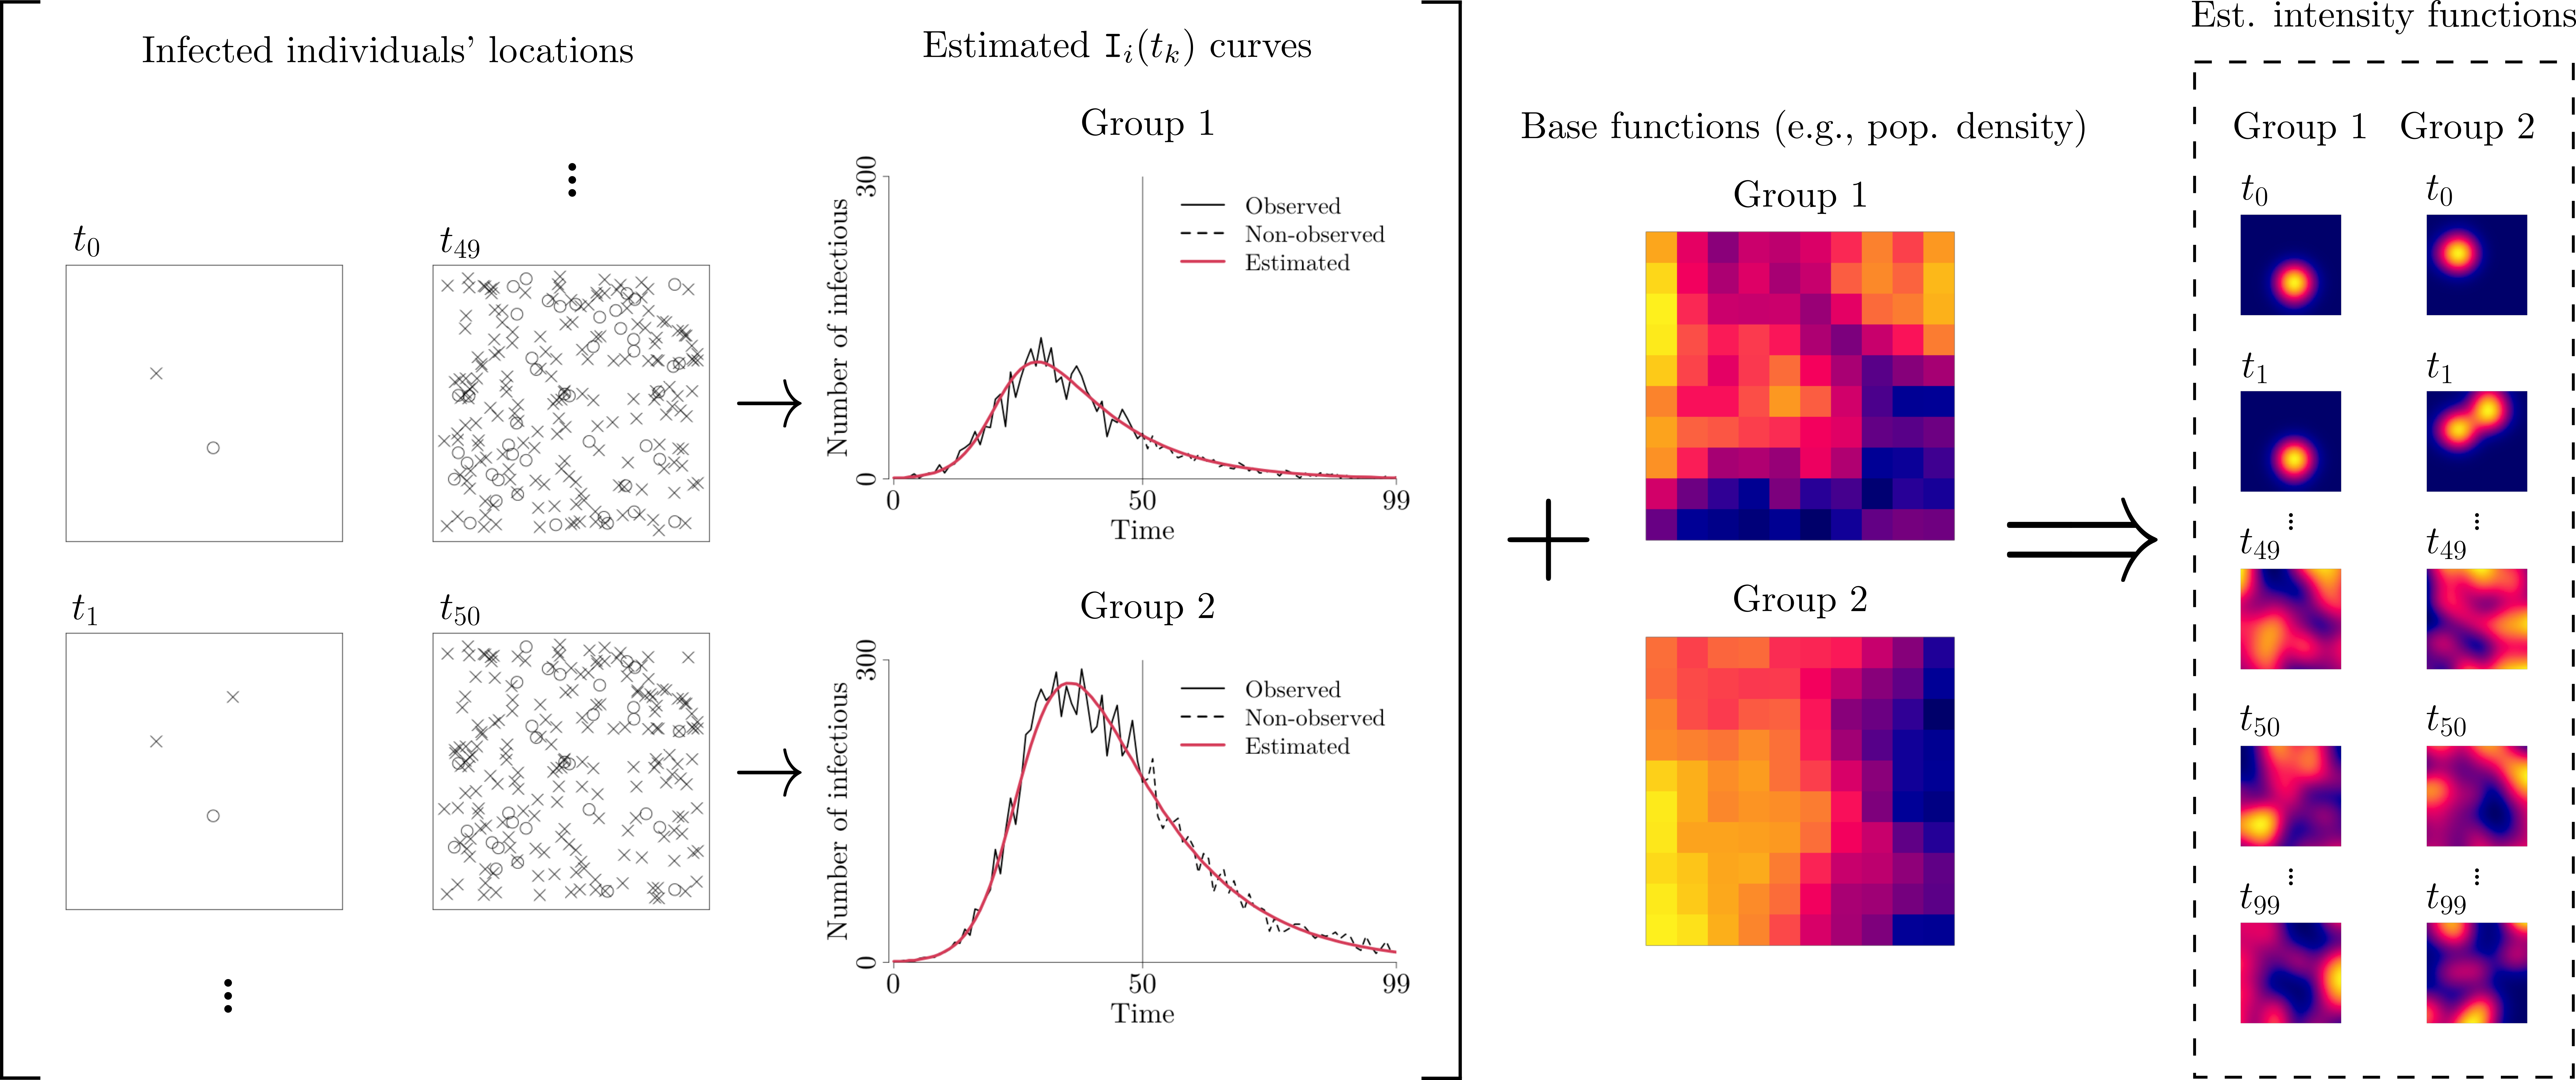
\includegraphics[width = 1\textwidth]{Images/diagram.png}
			\caption{\justifying Two-step\hspace{-1pt} spatio-temporal\hspace{-1pt} modeling\hspace{-1pt} approach for infectious in all groups.}
			\label{fig:diagramST}
		\end{figure}
		
	\end{frame}
	
	\begin{frame}[t]
		\frametitle{Temporal and Spatio-temporal modeling}
		\justifying
		
		\begin{columns}[T] % align columns
			\begin{column}{.48\textwidth}
				{\hfill{\large\textbf{SIR Model}}\hfill}\vspace{12pt}
				
				\justifying
				Let $\texttt{S}_i(t)$, $\texttt{I}_i(t)$, and $\texttt{R}_i(t)$ denote the counting curves for all compartments.
				{\footnotesize
				\begin{align*} 
					\frac{d\texttt{S}_i(t)}{dt} &= -\beta \texttt{S}_i(t) \sum_{\text{all}\,j}C_{ij}\cdot\frac{\texttt{I}_j(t)}{\texttt{N}_j} \\
					\frac{d\texttt{I}_i(t)}{dt} &= +\beta \texttt{S}_i(t) \sum_{\text{all}\,j}C_{ij}\cdot\frac{\texttt{I}_j(t)}{\texttt{N}_j} - \gamma \texttt{I}_i(t) \nonumber \\
					\frac{d\texttt{R}_i(t)}{dt} &= +\gamma \texttt{I}_i(t), \nonumber
				\end{align*}
				}%
				such that $C_{ij}$ is a contact matrix, $\texttt{N}_i(t) = \texttt{N}_i$, $\forall t$, and $\beta, \gamma > 0$.
			\end{column}%
			\hfill%
			\vline
			\hfill%
			\begin{column}{.60\textwidth}
				{\hfill{\large\textbf{LGCP Model}}\hfill}\vspace{12pt}
				
				\justifying
				Assuming we already estimated  $\texttt{I}_i(t_k)$, $\forall i, k$, the main model can be specified as follows
				{\footnotesize
				\begin{align*}
					\mathcal{N}_i(t_k)|\Lambda_i(\mathbf{u}; t_k) = \lambda_i(\mathbf{u}; t_k) &\sim \text{Po}\left(\int_{\mathcal{U}}\lambda_i(\mathbf{u}; t_k)d\mathbf{u}\right) \\
					\Lambda_i(\mathbf{u}; t_k) &= \mu_i(\mathbf{u}; t_k) \cdot \exp\{\zeta_i({\mathbf{u}; t_k})\} \nonumber \\
					\mu_i(\mathbf{u}; t_k) &= \lambda_{0, i}(\mathbf{u}; t_k) \cdot \texttt{I}_i(t_k) \nonumber \\ 
					\zeta_i(\mathbf{u}; t_k | \boldsymbol{\eta}_i) &\sim \text{GP} (\beta_{0, i}, \phi_i(h; t_k | \boldsymbol{\eta}_i)) \nonumber \\
					\boldsymbol{\eta}_i &\sim \text{priors}, \nonumber
				\end{align*}
				}%
				such that $\phi_i(h; t_k | \boldsymbol{\eta}_i)$ is a covariance function, and $\boldsymbol{\eta}_i$ is a vector of parameters.
			\end{column}%
		\end{columns}
		
	
		
	\end{frame}
		
	\begin{frame}[t]
		\frametitle{Data Simulation}
		\justifying
		
		We consider as a study region an area of approx. 3 km${}^{2}$ in São Paulo, Brazil. For such a region, we divided people into three age groups: 0--19, 20--59, 60+.
		
		\begin{figure}[!ht]
			\centering\vspace{-3pt}
			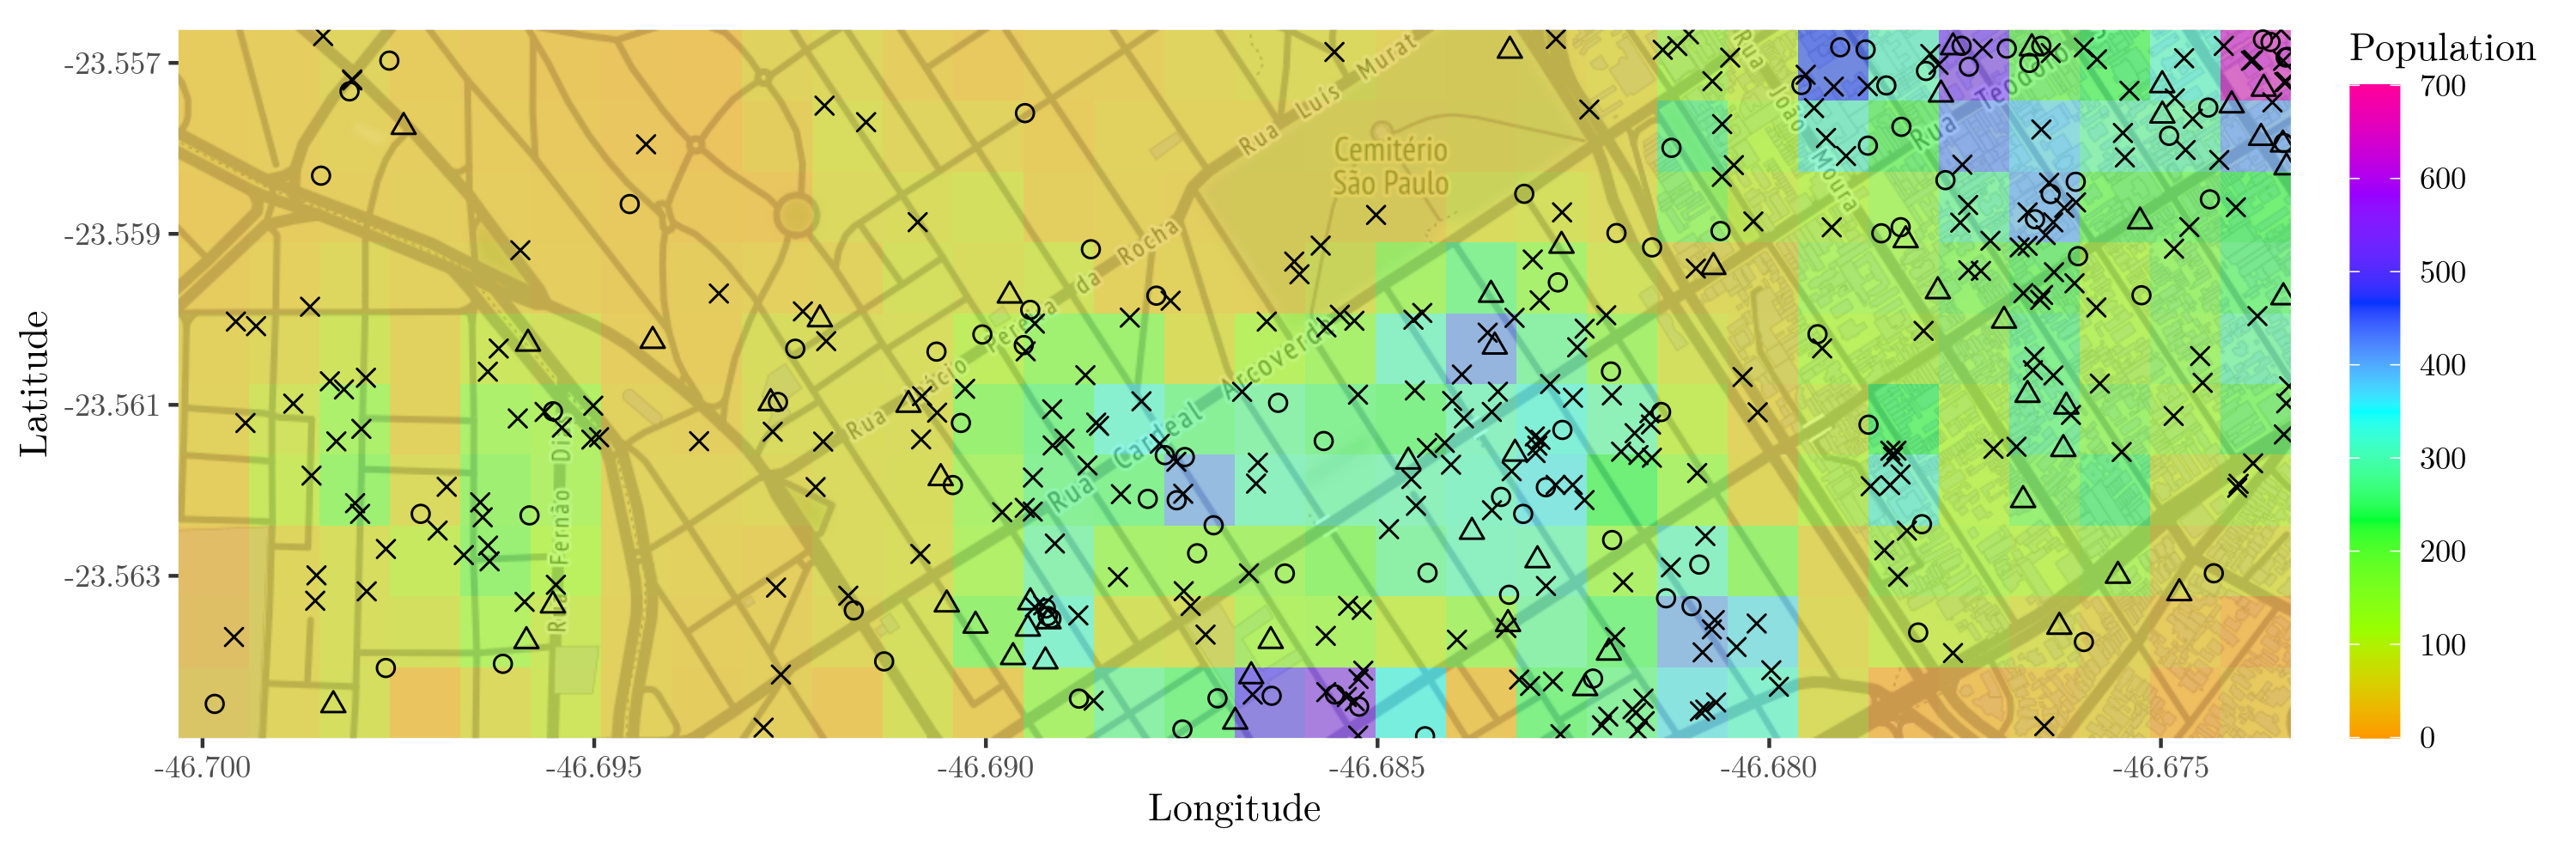
\includegraphics[width = 0.95\textwidth]{Images/map.png}\vspace{-12pt}
			\caption{\justifying Studied region in  São Paulo (Brazil) with the overlapped grid for the estimated population and infected individuals' locations.}1
			\label{fig:map}
		\end{figure}
		
	\end{frame}

	\begin{frame}[t]
		\frametitle{Model Assessment}
		\justifying
		
		Obtained errors for the null and alternative models under two different settings.\vspace{-3pt}
		\begin{figure}[!ht]
			\centering
			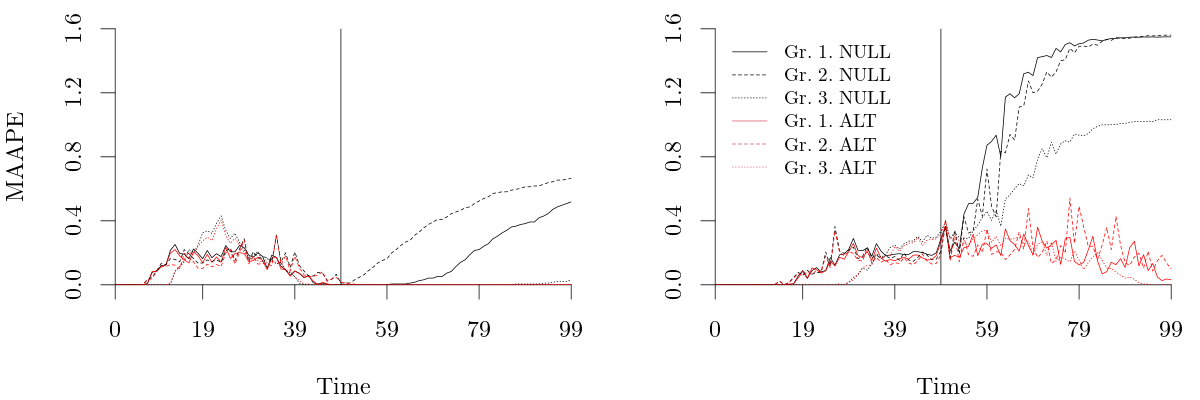
\includegraphics[width = 1\textwidth]{Images/computed_errors.png}\vspace{-6pt}
			\caption{\justifying Computed Mean Arctangent Absolute Percentage Error (MAAPE) for groups 0--19, 20--59, 60+. Models were fitted with data up to $t_{49}$ (vertical solid line).}
			\label{fig:computederrors}
		\end{figure}
		
	\end{frame}
	
\end{document}